
	\institute[]{UNIMONTES}
	\date[2017]{19 de Julho de 2017}
	% EDITAR ESSAS INFORMACOES (FIM)
	
	\begin{frame}
		\titlepage
	\end{frame}
	\begin{frame}
		\frametitle{Sum\'{a}rio}
		\tableofcontents%[pausesections]
	\end{frame}
	
%---------------------------------------------------------------------------
	% PRIMEIRA SECAO
	\section{Introdução, Motivação e Problematização}
%---------------------------------------------------------------------------

	% SLIDE	
	\begin{frame}
		\frametitle{Introdução}		
		\framesubtitle{Reconhecimento de Caracteres}		
		\begin{itemize}
			\item O reconhecimento inteligente de caracteres (ICR) é um segmento da Visão Computacional que tem como objetivo identificar os caracteres de diferentes fontes e caligrafias.
			\item A principal solução para problemas de ICR é o aprendizado de máquina, onde um algoritmo será treinado para dar soluções inteligentes para reconhecimento de caracteres.
		\end{itemize}	
	\end{frame}
	% SLIDE 	
	\begin{frame}
		\frametitle{Introdução}		
		\framesubtitle{Motivação}
		Diversos problemas dependem do reconhecimento de caracteres. Dentre eles, pode-se destacar os seguintes:
	 	\begin{itemize}
	 		\item Validação de assinatura manuscrita em documentos;
	 		\item Identificação de placas de trânsito por veículo autônomo;
	 		\item Inspeção de gravação do número de chassi em veículos;
	 		\item Portaria automatizada por meio de identificação do número da placa do carro.
	 	\end{itemize}
	\end{frame}
	% SLIDE	
\begin{frame}
	\frametitle{Introdução}		
	\framesubtitle{Problemática}		
	\begin{itemize}
		\item Entrentanto, como relata Menezes (2014), o reconhecimento de caracteres manuscritos ainda é um grande desafio da Visão Computacional.
		\item A dificuldade de identificar os caracteres manuscritos se dá pelas diversas caligrafias que podem ser utilizadas.
		\item Menezes (2014) relata também a dificuldade em definir os descritores para os caracteres, visto a complexidade em encontrar padrões nas amostras coletadas.
	\end{itemize}	
	\end{frame}

%SECAO 
\section{Objetivos}
	% SLIDE 	
	\begin{frame}
	\frametitle{Objetivos}
	%\framesubtitle{}
	Em busca de ampliar os conhecimentos sobre a temática e empreender alguma solução, este trabalho teve como objetivos:
	\begin{itemize}
		\item Aplicar os conhecimentos adquiridos durante o curso de Inteligência Computacional para confeccionar uma rede neural do Tipo Perceptron Multi-Camadas (MLP);
		\item Desenvolver um banco de dados próprio com caracteres numéricos manuscritos;
		\item Identificar caracteres manuscritos utilizando o algoritmo de treinamento \textit{Back-propagation};
		\item Verificar a eficiência do algoritmo \textit{Back-propagation} para reconhecimento de caracteres númericos manuscritos com base no banco de dados desenvolvido pelo estudo;
	\end{itemize}
	\end{frame}

	% SEÇÃO	
	\section{Metodologia}
	
	% SLIDE 	

	\begin{frame}
	\frametitle{Metodologia}
	\framesubtitle{Banco de Dados}
	Foi desenvolvido um banco de dados próprio a partir de amostras com caracteres manuscritos.
		\begin{figure}
		\centering
		\caption{Exemplo de amostra coletada com o algarismo 4.}
		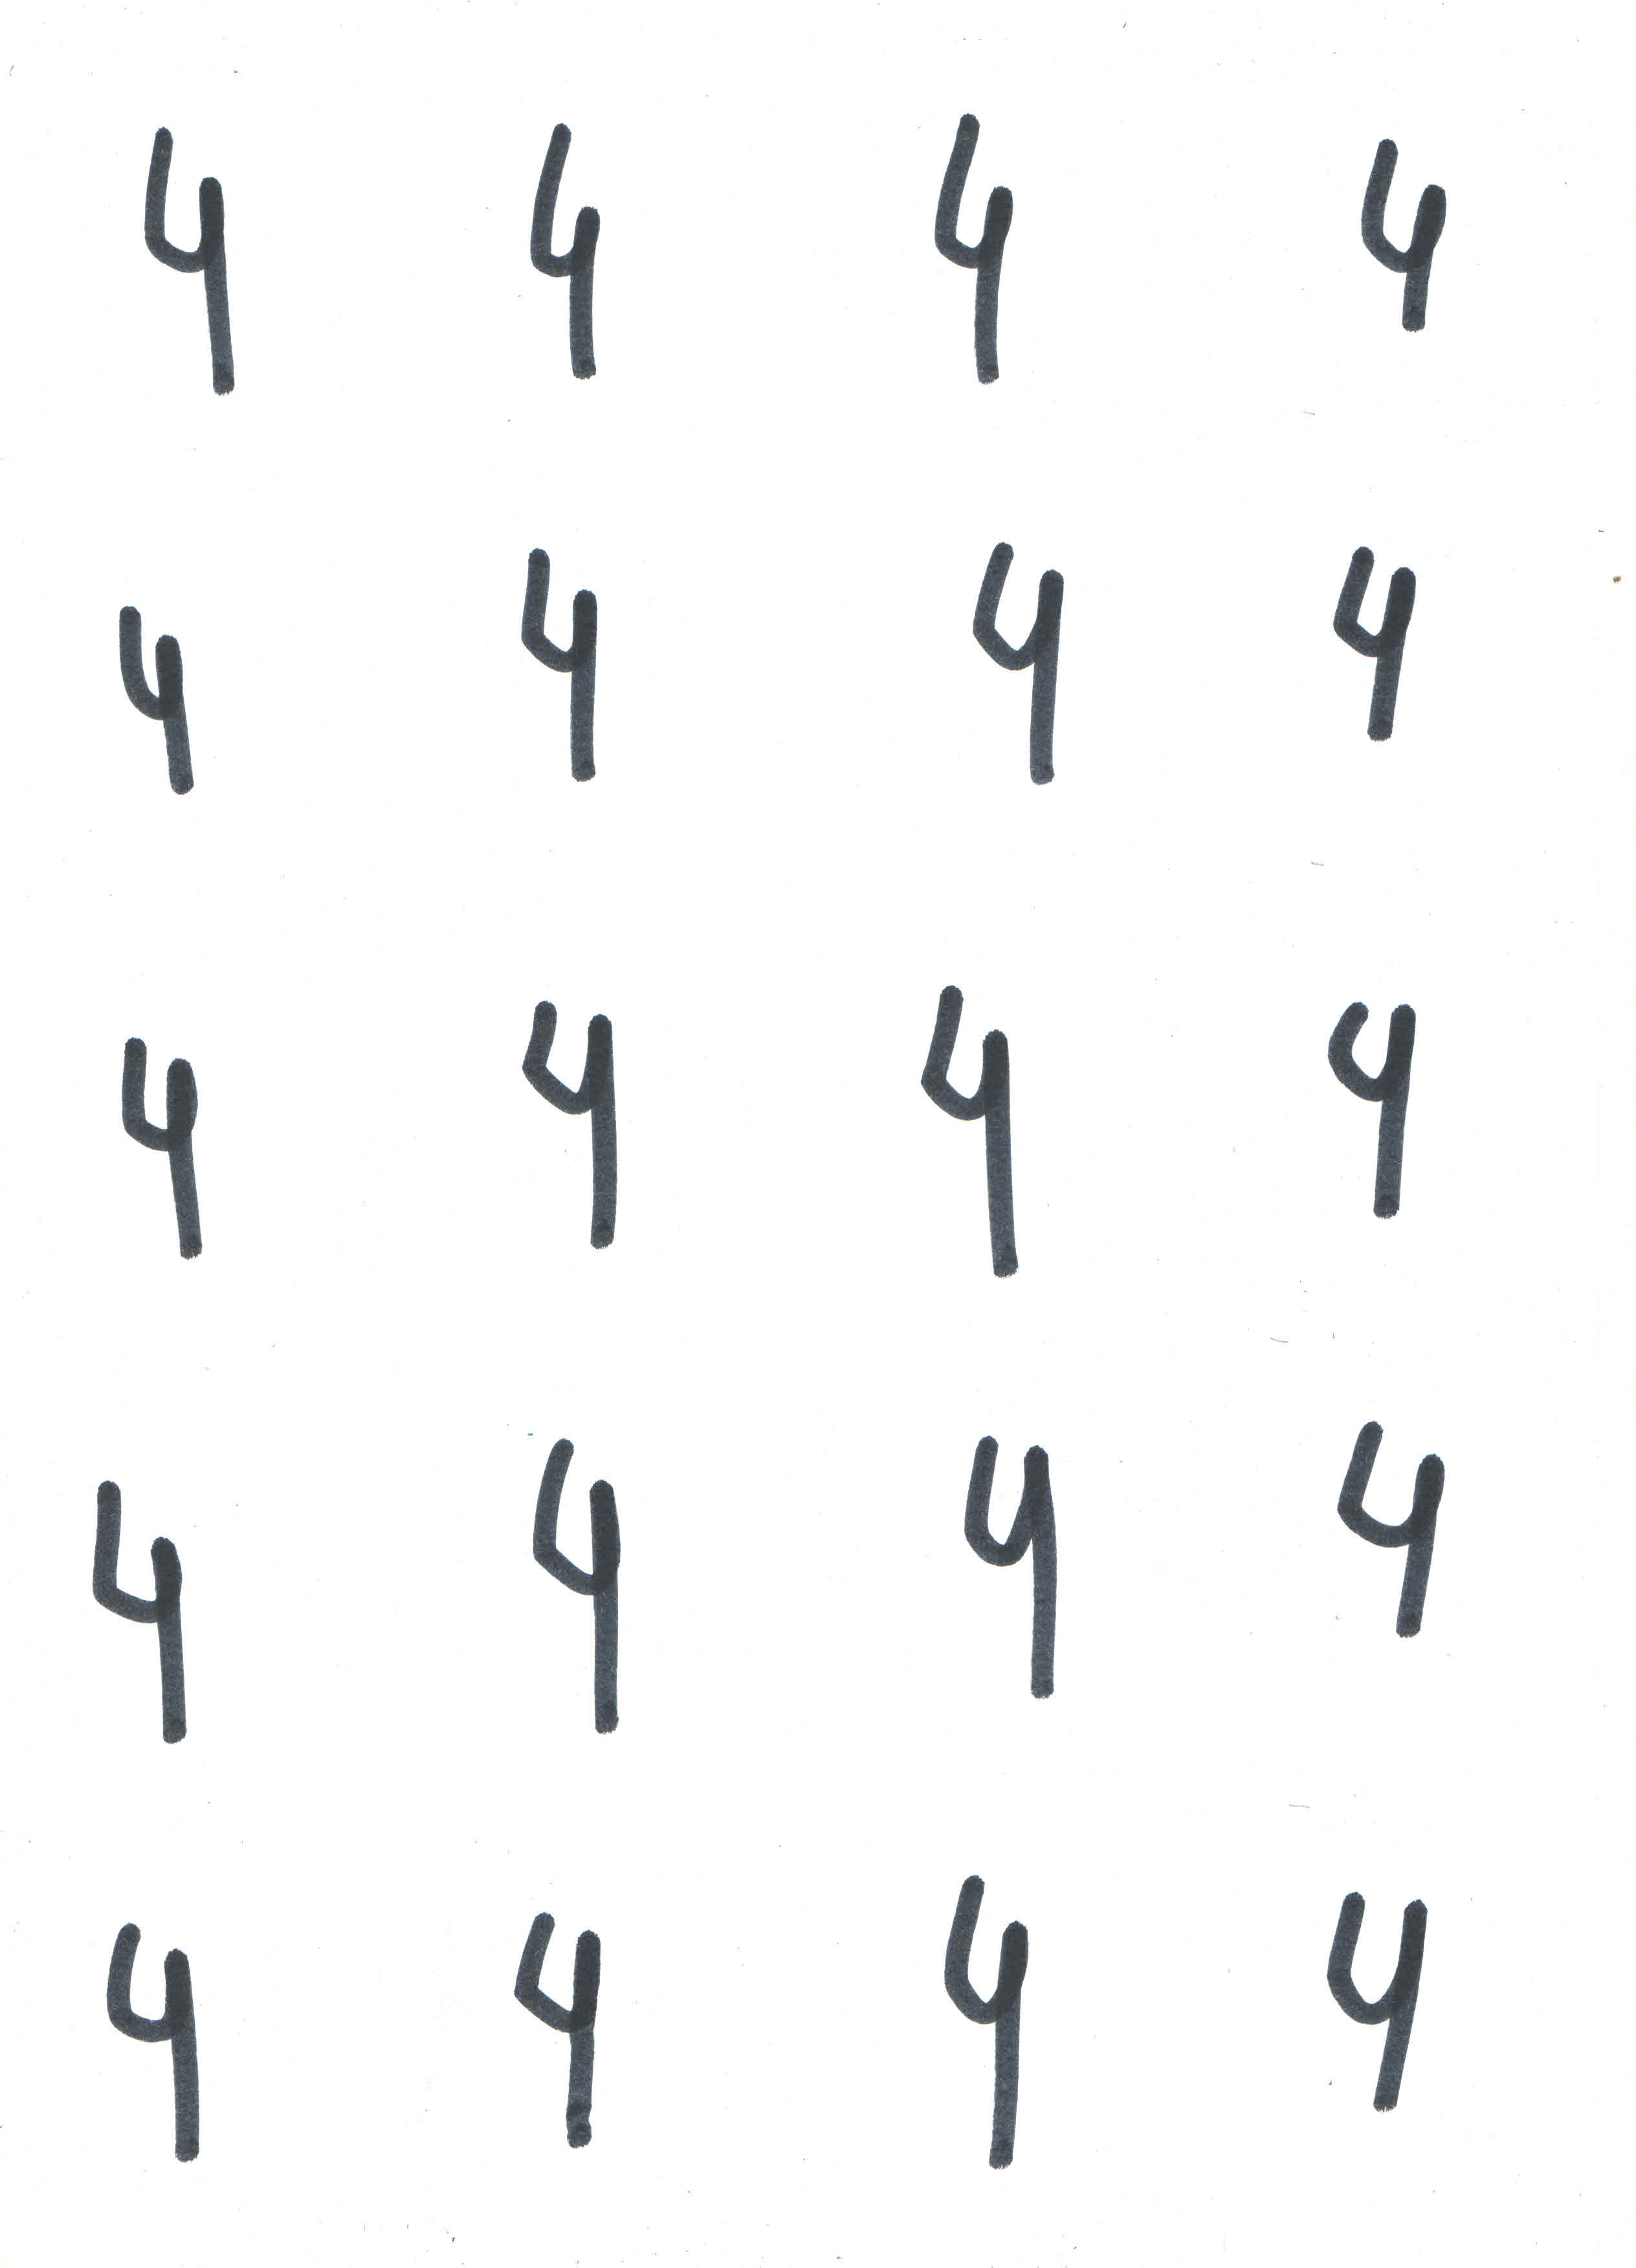
\includegraphics[width=.17\linewidth]{quatro1.jpg}\\
		{\scriptsize Fonte: Os autores}
		\label{figtextimg}
	\end{figure} 
	\end{frame}

	% SLIDE 	

	\begin{frame}
		\frametitle{Metodologia}
		\framesubtitle{Banco de Dados}
		\begin{itemize}
			\item Nas amostras, foram contemplados os caracteres de 0 a 9.
			\item Cada caractere numérico foi escrito manualmente 80 vezes em papel sulfite A4, totalizando 800 amostras. Após, foram feitos os scanners de todas as amostras.
			\item Cada imagem de amostra foi inicialmente adquirida no formato 700x500, e foi posteriormente redimensionada para 14x12, passando a possuir 168 pixels.
			\item Assim, cada amostra contém 168 variáveis de entrada, referentes a matriz de pixel de cada imagem de amostra e 4 variáveis de saída.
			
		\end{itemize}

	\end{frame}

	% SLIDE 	

\begin{frame}
	\frametitle{Metodologia}
	\framesubtitle{Banco de Dados}
	\begin{itemize}
		\item Após, as imagens sofreram conversão para escala de cinza e correção das intensidades de preto e branco.
		\item Com o banco de dados pronto, foram executados 2 treinamentos com os seguintes parâmetros:\vspace{0.3cm}
\\
Param.goal = $ 1x10^{-4} $\\
Param.mc = 0.9\\
Param.lr = 0.1\\
Param.show = 25
	\end{itemize}
	
\end{frame}
	% SLIDE 	

\begin{frame}
	\frametitle{Metodologia}
	\framesubtitle{Máquina de Testes}
	O treinamento foi executado em uma máquina com as seguintes configurações:
\begin{table}[H]
	\centering
	\caption{Configurações da Máquina de Testes.}
	\label{my-label}
	\begin{tabular}{@{}|l|l|@{}}
		\toprule
		\textbf{Parâmetro}  & \textbf{Configuração}            \\ \midrule
		Sistema Operacional & Windows 10 Pro                   \\ \midrule
		Processador         & Intel Core i7-5500U CPU 2.40 GHz \\ \midrule
		Memória RAM         & 8 GB                             \\ \bottomrule
	\end{tabular}
\end{table}
	
\end{frame}

	%SECAO 

	
		\section{Resultados}
	%SECAO 
	\begin{frame}
	\frametitle{Resultados}
	\framesubtitle{Treinamento}
	Os dois testes foram realizado com 101 amostras de validação em algoritmo MLP com \textit{momentum} e função de ativação senoidal.
	\begin{itemize}
		\item Para o primeiro teste, o banco de dados contava apenas com as 80 amostras inicialmente inseridas.
		\item Este primeiro teste conquistou 84 acertos e 17 erros, com eficiência de 83,16\%. Ele foi concluído em 2hs 39min 58s, com 500.000 épocas de treinamento e erro final de 0,0295.
		
	\end{itemize}

	\end{frame}	


\begin{frame}
	\frametitle{Resultados}
	\framesubtitle{Treinamento}

	\begin{itemize}
		\item Entrentanto, para o segundo teste, com o intuito de melhorar a eficiência do banco de dados, foi aumentado o número de amostras de cada caractere para 180.
		\item O segundo teste, por sua vez, obteve 98 acertos e 3 erros, totalizando 97\% de eficiência. Esse teste terminou em 3hs 21min 48s, com 500.000 épocas de treinamento e erro final de 0,0183.
		
	\end{itemize}
	
\end{frame}	
	
	
	\begin{frame}
		\frametitle{Resultados}
		\framesubtitle{Treinamento}
		Após os treinamentos, foram verificados os seguintes resultados:
			\begin{figure}[H]
			\centering
			\caption{Telas obtidas após o treinamento 1 e 2.}
			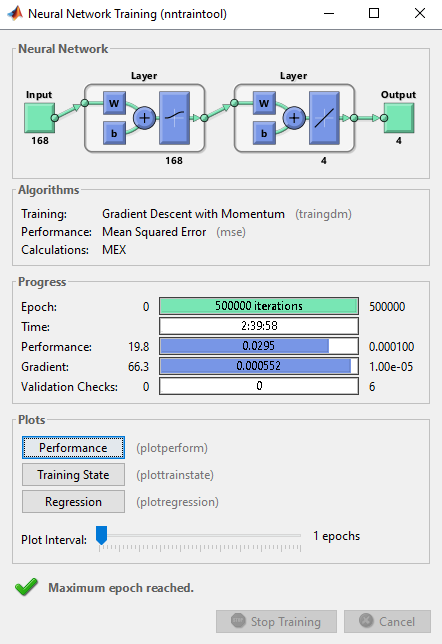
\includegraphics[width=0.22 \linewidth]{treinamento1.png}
			\quad
			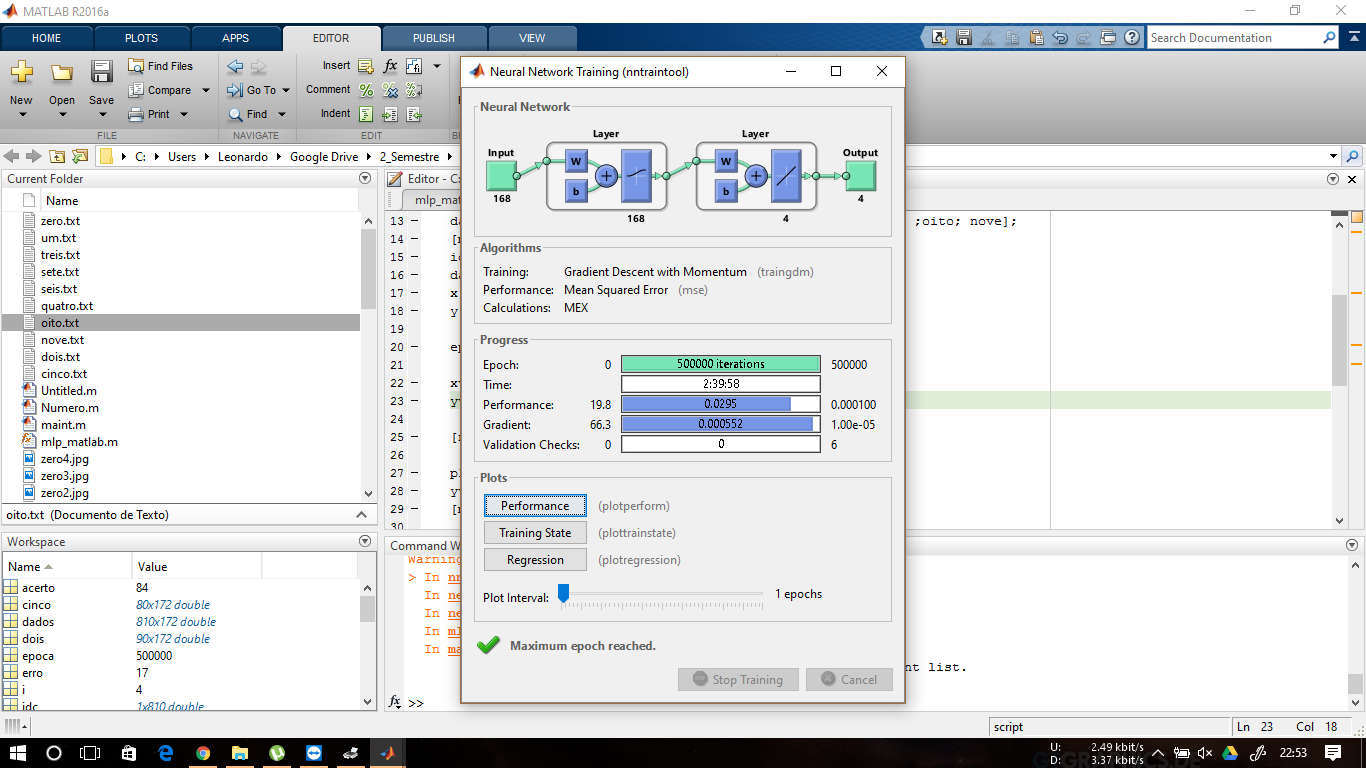
\includegraphics[width=0.22 \linewidth]{treinamento.png}\\
			{\scriptsize Fonte: Os autores}
			\label{view}
		\end{figure} 
	\end{frame}

	\begin{frame}
	\frametitle{Resultados}
	\framesubtitle{Treinamento}
	Os resultados de cada treinamento podem ser contemplados nos gráficos abaixo:
	\begin{figure}
		\centering
		\caption{Gráficos do 1º e 2º treinamentos do algoritmo com o erro quadrático médio em função do número de épocas.}
		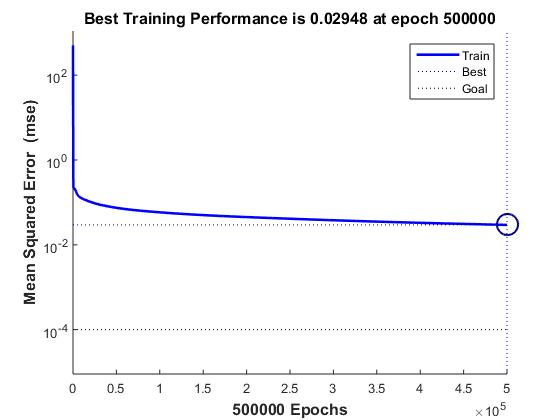
\includegraphics[width=0.37 \linewidth]{grafico1.jpg}
		\quad
		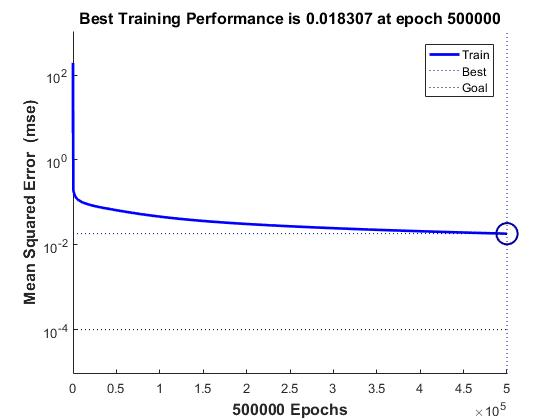
\includegraphics[width=0.37 \linewidth]{grafico.jpg}\\
		{\scriptsize Fonte: Os autores}
		\label{figtextimg}
	\end{figure} 

\begin{figure}
	\centering
	\caption{Gráficos do 3° treinamentos do algoritmo com o erro quadrático médio em função do número de épocas.}
	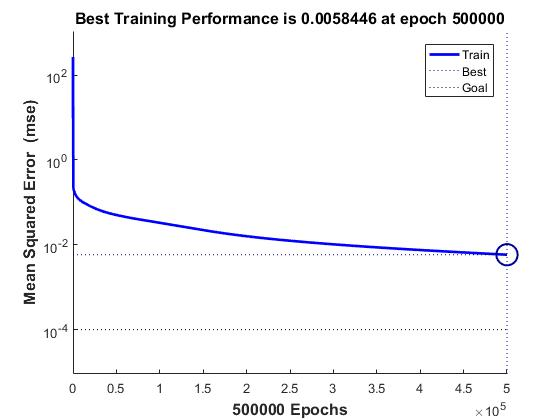
\includegraphics[width=0.37 \linewidth]{grafico100.jpg}
		{\scriptsize Fonte: Os autores}
	\label{figtextimg}
\end{figure} 
	
\end{frame}
\section{Considerações Finais}
\begin{frame}
	\frametitle{Considerações Finais}
	\begin{itemize}
		\item Ao final dos experimentos, foi notável a capacidade de aprendizado e generalização obtida pelo MLP por meio do algoritmo de treinamento \textit{Back-propagation}, conquistando o objetivo da pesquisa, que era identificar caracteres manuscritos utilizando esse algoritmo.
		\item Também foi notável a diferença entre os resultados do primeiro para o segundo teste, demonstrando que a quantidade de amostras influencia na eficiência da rede neural desenvolvida.
		\item Não obstante, pesquisas adicionais podem ser feitas com o intuito de melhorar ainda mais a taxa de acerto na validação do algoritmo com base no banco de dados proposto por esse estudo utilizando outros parâmetros para treinamento, inserção de novas caligrafias e o consequente aumento da quantidade de amostras. 
	\end{itemize} 

\end{frame}


%---------------------------------------------------------------------------
	%SECAO DE REFERENCIAS
	\section{Refer\^{e}ncias bibliogr\'{a}ficas}
%---------------------------------------------------------------------------
	% SLIDE  - REFERENCIAS
	\begin{frame}
		\frametitle{Refer\^{e}ncias Bibliogr\'{a}ficas}
		\begin{enumerate}
			\item BERG, Alexandre Cruz; MULLER, Daniel Nehme; ENGEL, Paulo Martins. \textbf{Reconhecimento de Caracteres Usando Redes Neurais}. Universidade Federal do Rio Grande do Sul. Porto Alegre: 1993
			\item LIMA JÚNIOR, H. P. \textbf{Aplicação de Redes Neurais no reconhecimento de letras em placas de veículos automotores brasileiros}. Centro Brasileiro de Pesquisas Físicas: 2000.
		\end{enumerate}
	\end{frame}


	%---------------------------------------------------------------------------
\end{document}
